
\chapter{Exercise 10}
\label{cha:ugeopgave-10}

The purpose of this exercise is to become familiar with the concepts behind environment mapping and bump mapping. We will use environment mapping to simulate mirrors and glass and in the process learn to use cube maps, reflection/refraction functions and Schlick's approximation. Finally we will apply bump mapping to a sphere to add small scale details.

\section{Part 1}
\label{sec:del-1}

After following descriptions described in exercise description document, I build the skymap. A screen capture of executing program can be seen in Figure \ref{fig:10-1}.

\begin{figure}[hp]
\centering
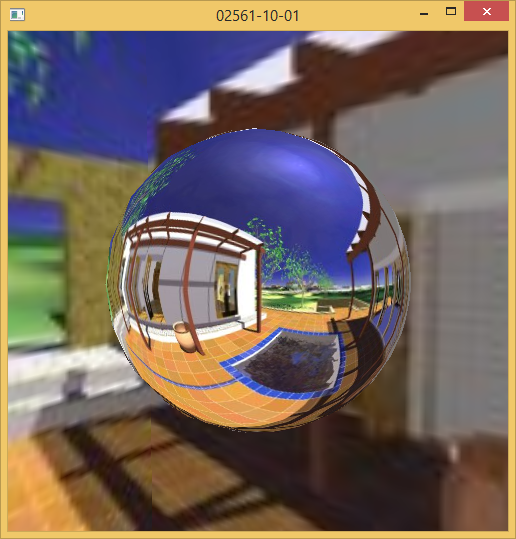
\includegraphics[width=8cm]{../Screenshots/ex-10/1.png}
\caption{Skybox and sphere with mirror shader}
\label{fig:10-1}
\end{figure}

\section{Part 2}
\label{sec:del-2}

After following descriptions described in exercise description document, I manage to implement mirror shader. You can see a screenshot of this shader in Figure \ref{fig:10-1}.

\section{Part 3}
\label{sec:del-3}

After following descriptions described in exercise description document, I manage to implement glass shader. To get fresnel term, which is needed in shader calculations, I use schlick's approximation. You can see the GLSL code fragment that calculates fresnel term below.
\begin{lstlisting}

	float R0 = pow(abs((air-glass)/(air+glass)),2.0);
	float R = R0 + (1-R0)*pow(1.-max(dot(n, -i),0.), 5);

\end{lstlisting}

\noindent
where \emph{air} is refracting index of air, \emph{glass} is refracting factor of index, n is normal vector of the fragment (pixel), i is incident vector of the fragment.

You can see a screenshot of this shader in Figure \ref{fig:10-3}.

\begin{figure}[hp]
\centering
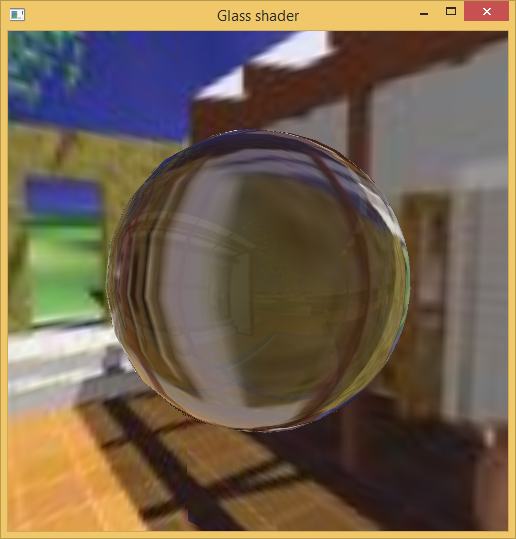
\includegraphics[width=8cm]{../Screenshots/ex-10/3.png}
\caption{Glass shader}
\label{fig:10-3}
\end{figure}


\section{Part 4}
\label{sec:del-4}


After following descriptions described in exercise description document, I manage to implement a bump-map on our sphere. 

You can see a screenshot of this shader in Figure \ref{fig:10-4}.


\begin{figure}[hp]
\centering
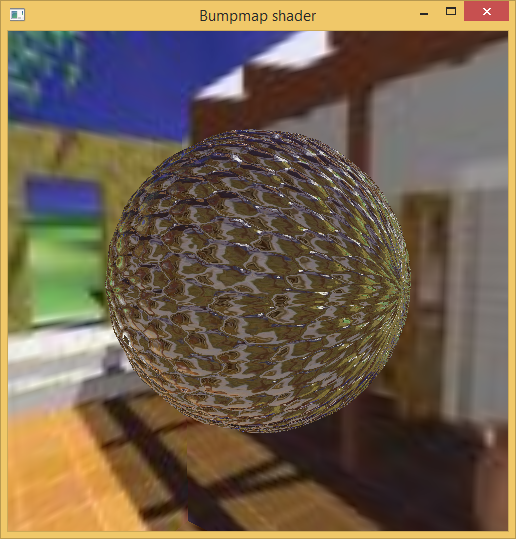
\includegraphics[width=8cm]{../Screenshots/ex-10/4.png}
\caption{Bump-mapping on a sphere}
\label{fig:10-4}
\end{figure}


\section{Part 5}
\label{sec:del-5}
 
 To simulate this, do three lookups in the cube map, one for red, green, and blue, each with different index of refraction, when computing the refraction color. The refraction indexes of the colors in glass are given as:\\
 
 \noindent
 $n_{red} = 1.56 $ \\
 $n_{green} = 1.615 $ \\
 $n_{blue} = 1.63 $ \\
 $n_{glass} = 1.615 $ (used in calculation of fresnel term) \\
 
 The resulting screenshot can be seen in Figure \ref{fig:10-5}. 


\begin{figure}[hp]
\centering
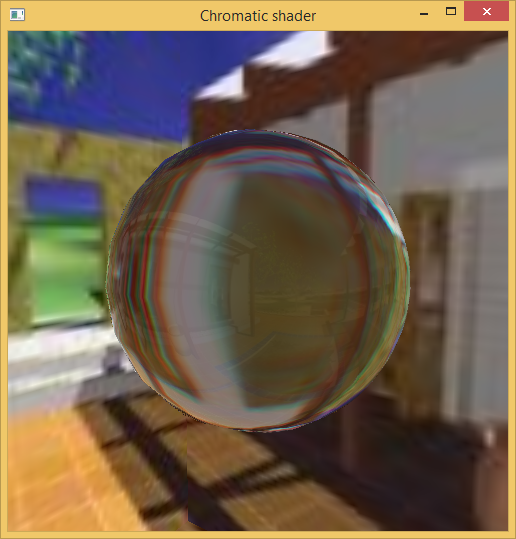
\includegraphics[width=8cm]{../Screenshots/ex-10/5.png}
\caption{Chromatic glass shader}
\label{fig:10-5}
\end{figure}
%%% Local Variables:
%%% mode: latex
%%% TeX-master: "report_main"
%%% End: 